\documentclass[convert={imagemagick, density=1024}]{standalone}
\usepackage{amsmath, amsthm, amsfonts}
\usepackage{tikz-cd, kotex}
\usepackage{../../.preamble/quiver}
\usepackage{../../.preamble/Operators}
\usetikzlibrary{arrows.meta}
\begin{document}

%% Pic ↪ Cl commutative diagram (Toric_Divisors_and_Line_Bundles-1.png)
\begin{tikzcd}[column sep=large, row sep=large]
0 \rar & M \rar \dar[equal] & \CaDiv_T(X_\Sigma) \rar \dar[hook] & \Pic(X_\Sigma) \rar \dar[hook] & 0 \\
0 \rar & M \rar             & \Div_T(X_\Sigma)   \rar           & \Cl(X_\Sigma)   \rar           & 0
\end{tikzcd}

\end{document}

%% P^2 fan: three 2-dim cones generated by e_1, e_2, -e_1-e_2 (Toric_Varieties-1.png)
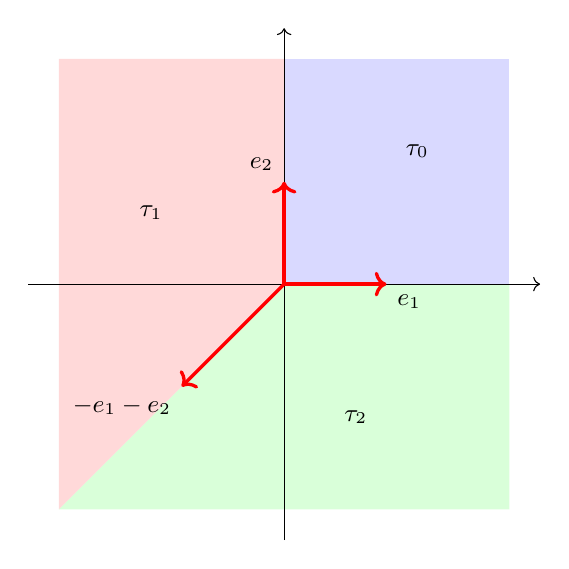
\begin{tikzpicture}[scale=1.3, every node/.style={font=\small}]
  % Three 2-dim cones filled
  \fill[blue!15]  (0,0) -- (2.2,0) -- (2.2,2.2) -- (0,2.2) -- cycle;
  \fill[red!15]   (0,0) -- (0,2.2) -- (-2.2,2.2) -- (-2.2,-2.2) -- cycle;
  \fill[green!15] (0,0) -- (2.2,0) -- (2.2,-2.2) -- (-2.2,-2.2) -- cycle;

  % Axes (black)
  \draw[->, thin, black] (-2.5,0) -- (2.5,0);
  \draw[->, thin, black] (0,-2.5) -- (0,2.5);

  % Three primitive generators (red)
  \draw[->, very thick, red] (0,0) -- (1,0)   node[below right, black] {$e_1$};
  \draw[->, very thick, red] (0,0) -- (0,1)   node[above left, black]  {$e_2$};
  \draw[->, very thick, red] (0,0) -- (-1,-1) node[below left, black]  {$-e_1-e_2$};

  % Cone labels
  \node at (1.3, 1.3)  {$\tau_0$};
  \node at (-1.3, 0.7) {$\tau_1$};
  \node at (0.7, -1.3) {$\tau_2$};
\end{tikzpicture}
